%!TEX root = main.tex
\section{Supplementary Simulation Results}
%%%%%%%%%%%%%%%%%%%%%%%%%%%%%%%%%%%%%%%%
\begin{figure}
\centering
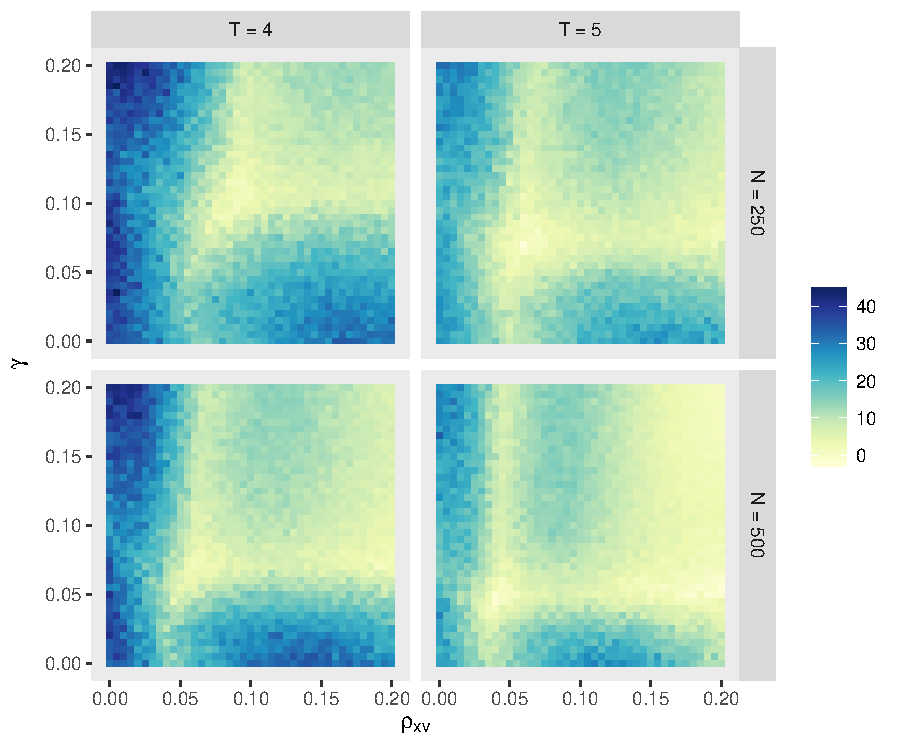
\includegraphics[scale = 0.8]{./simulations/DynamicPanel/results/Dpanel_GFIC_RMSE_rel_oracle}
\caption{GFIC RMSE relative to Oracle}
\end{figure}
%%%%%%%%%%%%%%%%%%%%%%%%%%%%%%%%%%%%%%%%
\begin{figure}
\centering
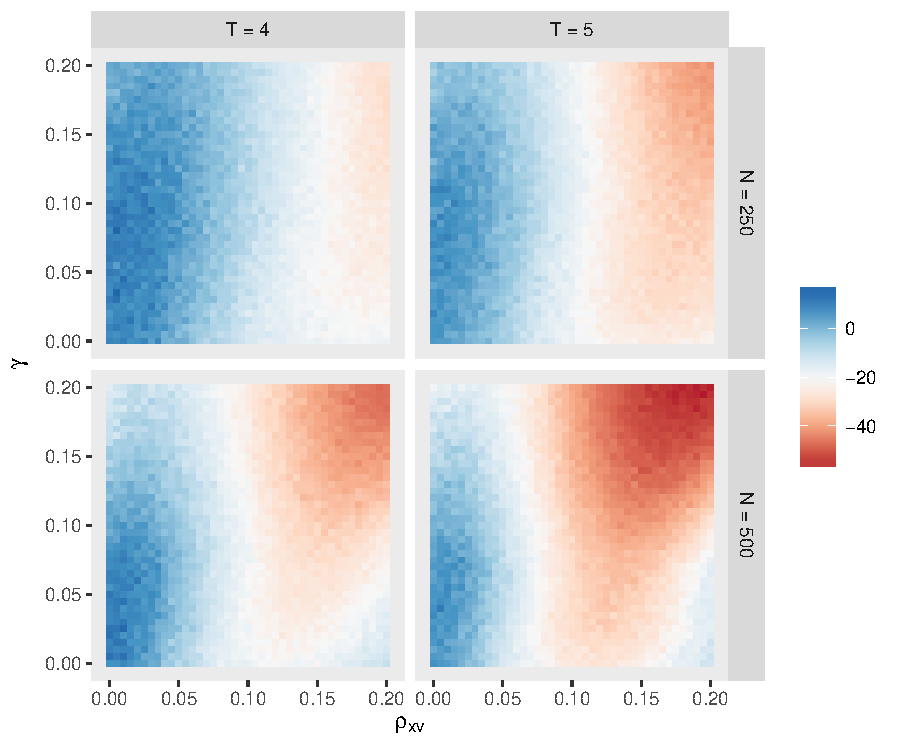
\includegraphics[scale = 0.8]{./simulations/DynamicPanel/results/Dpanel_GFIC_RMSE_rel_AIC}
\caption{GFIC RMSE relative to AIC}
\end{figure}
%%%%%%%%%%%%%%%%%%%%%%%%%%%%%%%%%%%%%%%%
\begin{figure}
\centering
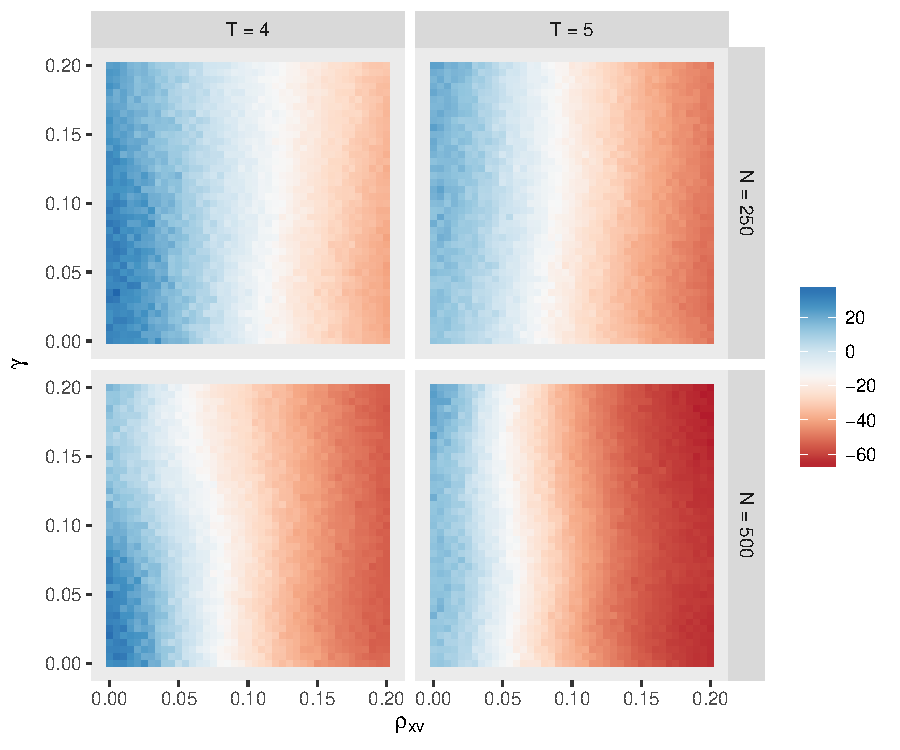
\includegraphics[scale = 0.8]{./simulations/DynamicPanel/results/Dpanel_GFIC_RMSE_rel_BIC}
\caption{GFIC RMSE relative to BIC}
\end{figure}
%%%%%%%%%%%%%%%%%%%%%%%%%%%%%%%%%%%%%%%%
\begin{figure}
\centering
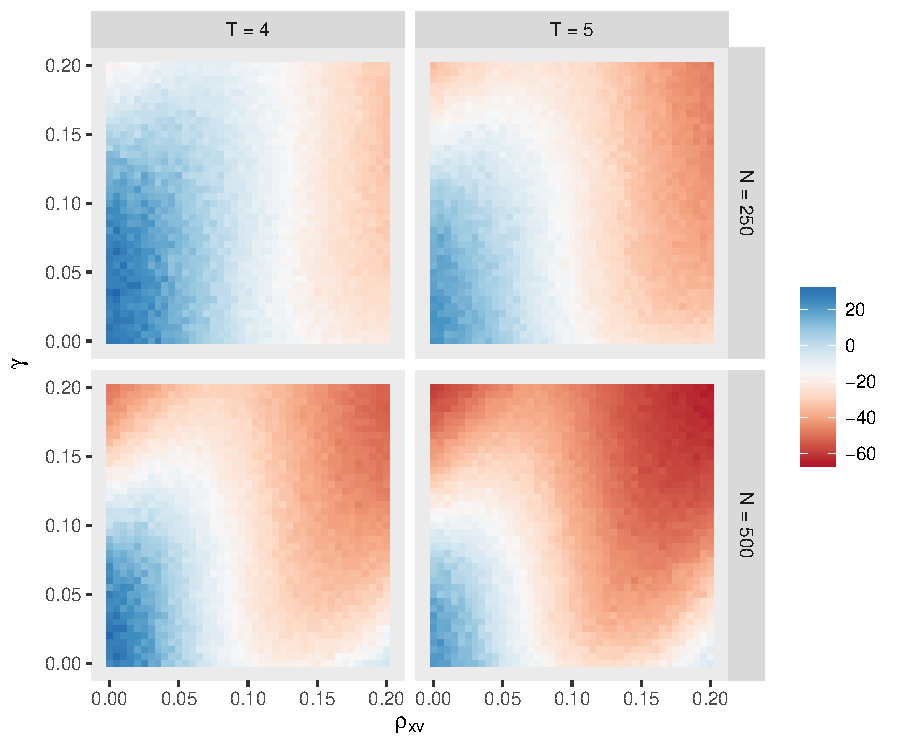
\includegraphics[scale = 0.8]{./simulations/DynamicPanel/results/Dpanel_GFIC_RMSE_rel_J5}
\caption{GFIC RMSE relative to J5}
\end{figure}
%%%%%%%%%%%%%%%%%%%%%%%%%%%%%%%%%%%%%%%%
\begin{figure}
\centering
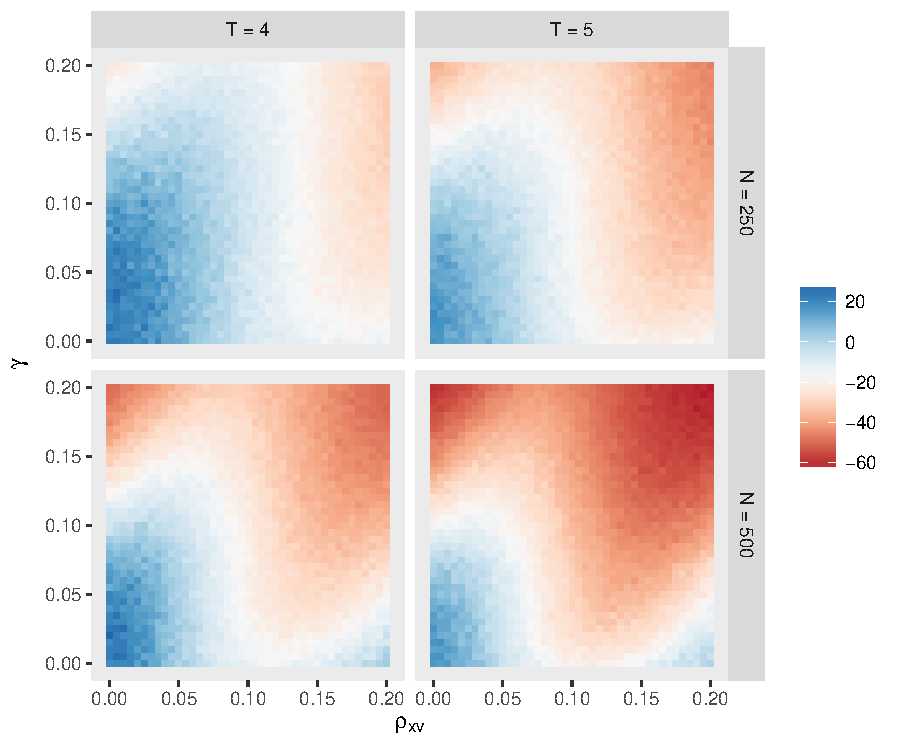
\includegraphics[scale = 0.8]{./simulations/DynamicPanel/results/Dpanel_GFIC_RMSE_rel_J10}
\caption{GFIC RMSE relative to J10}
\end{figure}

%%%%%%%%%%%%%%%%%%%%%%%%%%%%%%%%%%%%%%%%
\begin{figure}
\centering
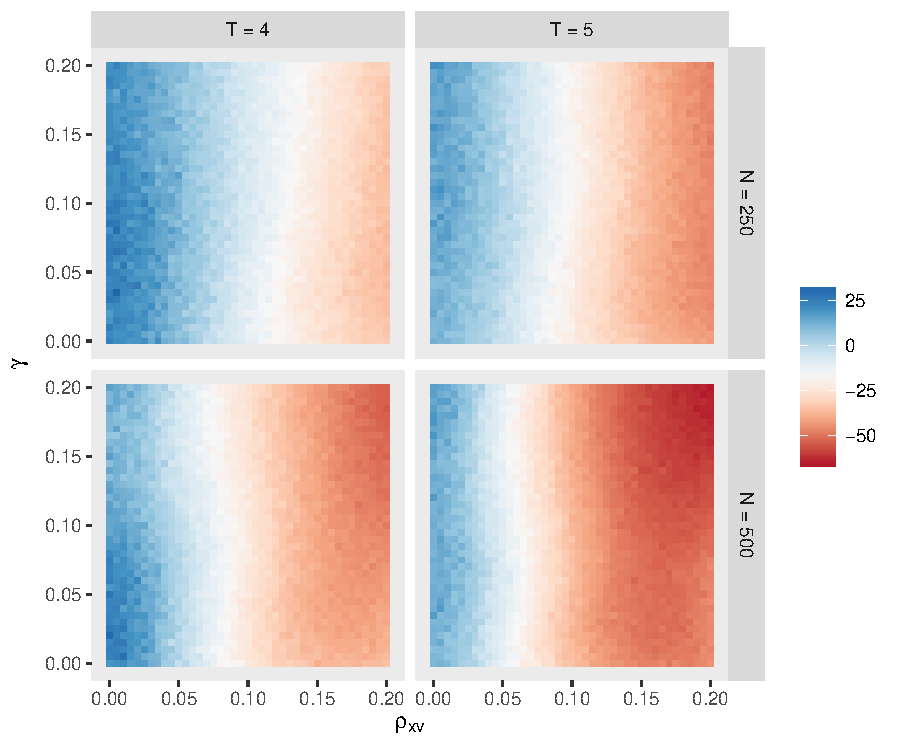
\includegraphics[scale = 0.8]{./simulations/DynamicPanel/results/Dpanel_GFIC_RMSE_rel_HQ}
\caption{GFIC RMSE relative to HQ}
\end{figure}

%%%%%%%%%%%%%%%%%%%%%%%%%%%%%%%%%%%%%%%%
\begin{sidewaystable}
  \footnotesize
  \centering
  \begin{tabular}{cccc|cccc|cccc|cccc|cccc} 
 \hline \hline 
\multicolumn{4}{c}{}&\multicolumn{4}{c}{Oracle}&\multicolumn{4}{c}{GFIC}&\multicolumn{4}{c}{J-test 10\%}&\multicolumn{4}{c}{GMM-HQ}\\ 
 \hline
 &  &  & $\rho$ & 0 & 0.05 & 0.1 & 0.15 & 0 & 0.05 & 0.1 & 0.15 & 0 & 0.05 & 0.1 & 0.15 & 0 & 0.05 & 0.1 & 0.15 \\
$T$ & $N$ & $\gamma$ &  &  &  &  &  &  &  &  &  &  &  &  &  &  &  &  &  \\
4 & 250 & 0 &  & 42 & 49 & 52 & 52 & 57 & 60 & 62 & 67 & 46 & 53 & 68 & 77 & 46 & 55 & 70 & 88 \\
 &  & 0.05 &  & 43 & 54 & 58 & 56 & 60 & 62 & 67 & 69 & 49 & 56 & 73 & 86 & 48 & 56 & 74 & 93 \\
 &  & 0.1 &  & 47 & 57 & 71 & 70 & 66 & 67 & 74 & 75 & 58 & 63 & 78 & 94 & 53 & 60 & 78 & 97 \\
 &  & 0.15 &  & 53 & 62 & 74 & 75 & 71 & 75 & 78 & 82 & 73 & 75 & 86 & 101 & 59 & 69 & 84 & 102 \\
 & 500 & 0 &  & 30 & 37 & 36 & 36 & 40 & 43 & 48 & 48 & 34 & 43 & 55 & 57 & 34 & 44 & 63 & 79 \\
 &  & 0.05 &  & 31 & 45 & 44 & 43 & 43 & 47 & 51 & 49 & 36 & 48 & 63 & 69 & 34 & 47 & 66 & 82 \\
 &  & 0.1 &  & 36 & 47 & 50 & 50 & 45 & 53 & 56 & 54 & 49 & 56 & 71 & 82 & 40 & 53 & 73 & 89 \\
 &  & 0.15 &  & 36 & 48 & 52 & 50 & 50 & 56 & 59 & 56 & 73 & 69 & 81 & 95 & 43 & 60 & 79 & 98 \\
5 & 250 & 0 &  & 36 & 44 & 44 & 45 & 45 & 48 & 54 & 56 & 38 & 46 & 61 & 71 & 40 & 50 & 69 & 86 \\
 &  & 0.05 &  & 38 & 50 & 51 & 48 & 48 & 52 & 56 & 55 & 42 & 52 & 66 & 78 & 42 & 52 & 70 & 89 \\
 &  & 0.1 &  & 42 & 53 & 55 & 55 & 51 & 57 & 61 & 58 & 50 & 59 & 74 & 88 & 45 & 56 & 74 & 94 \\
 &  & 0.15 &  & 44 & 52 & 58 & 57 & 55 & 61 & 65 & 64 & 67 & 68 & 82 & 96 & 47 & 58 & 80 & 98 \\
 & 500 & 0 &  & 27 & 31 & 32 & 32 & 33 & 36 & 40 & 38 & 29 & 38 & 49 & 46 & 30 & 41 & 60 & 73 \\
 &  & 0.05 &  & 29 & 39 & 38 & 38 & 35 & 40 & 40 & 38 & 32 & 44 & 57 & 61 & 31 & 44 & 63 & 77 \\
 &  & 0.1 &  & 31 & 40 & 39 & 40 & 37 & 44 & 44 & 41 & 44 & 53 & 69 & 78 & 33 & 48 & 70 & 86 \\
 &  & 0.15 &  & 31 & 42 & 39 & 40 & 38 & 45 & 44 & 42 & 70 & 66 & 78 & 90 & 33 & 53 & 76 & 94 \\
\hline
\end{tabular}
  \caption{RMSE values multiplied by 1000}
\end{sidewaystable}

%%%%%%%%%%%%%%%%%%%%%%%%%%%%%%%%%%%%%%%%

